%!TEX root = paper.tex
%%%%%%%%%%%%%%%%%%%%%%%%%%%%%%%%%%%%%%%%%%%%%%%%%%%%%%%%%%%%%%%%%%%%%%%%%%%%%%%%
\section{Background}
\label{sec:background}

Some fundamental gaming terms and concepts need to be introduced first. At their core video games are essentially feedback-directed real-time simulators. The game reads player input, updates the game state, and renders new screen contents. This loop repeats as long as the game is running. While the three parts are interrelated, and every component provides some form of input to the next, they may still proceed at their own intrinsic paces. The \textit{tickrate} governs the frequency of game state updates, and the \textit{framerate} determines the update rate of the output image. Examples for the tickrates of popular networked games and their servers include \SI{64}{\hertz} or \SI{128}{\hertz} for \textsc{CS:GO}, \SI{20}{\hertz} for \textsc{Minecraft}, or \SI{30}{\hertz} for \textsc{Dota 2}. Below the threshold of \textit{apparent motion} (about $16.67$ frames per per second) objects will appear as two distinct objects between two consecutive still images. Video games are more flexible but also much more demanding on the framerate than traditional media, whose framerates hover at the lower end of motion perception. Video games have to target higher framerates, e.g., \SI{30}{\hertz}, \SI{60}{\hertz}, or even \SI{120}{\hertz}. This enables smoother camera and object movement and help increase the interactivity and reactivity as video games constantly require input on short time scales to which the game reacts and displays the feedback. Lag is a critically important factor for almost all games, as it governs the reaction time to in-game events and such the chance of success. But this lag is often described solely on the basis of the \textit{network delay} in an online game, neglecting other components that contribute to the lag, including the input device, the time to sample and process the input, the game engine and server and their tickrates, frame rendering time, and ultimately the time to display the frame on the monitor. Only if all sources are factored in, the complete \gls{E2E} lag is captured, which can be highly variable. Fig.~\ref{fig:measurement-methods} depicts three distinct vantage points to measure portions of \gls{E2E} lag. Only external methods can capture the complete lag.

\begin{figure}[!t]
    \centering
    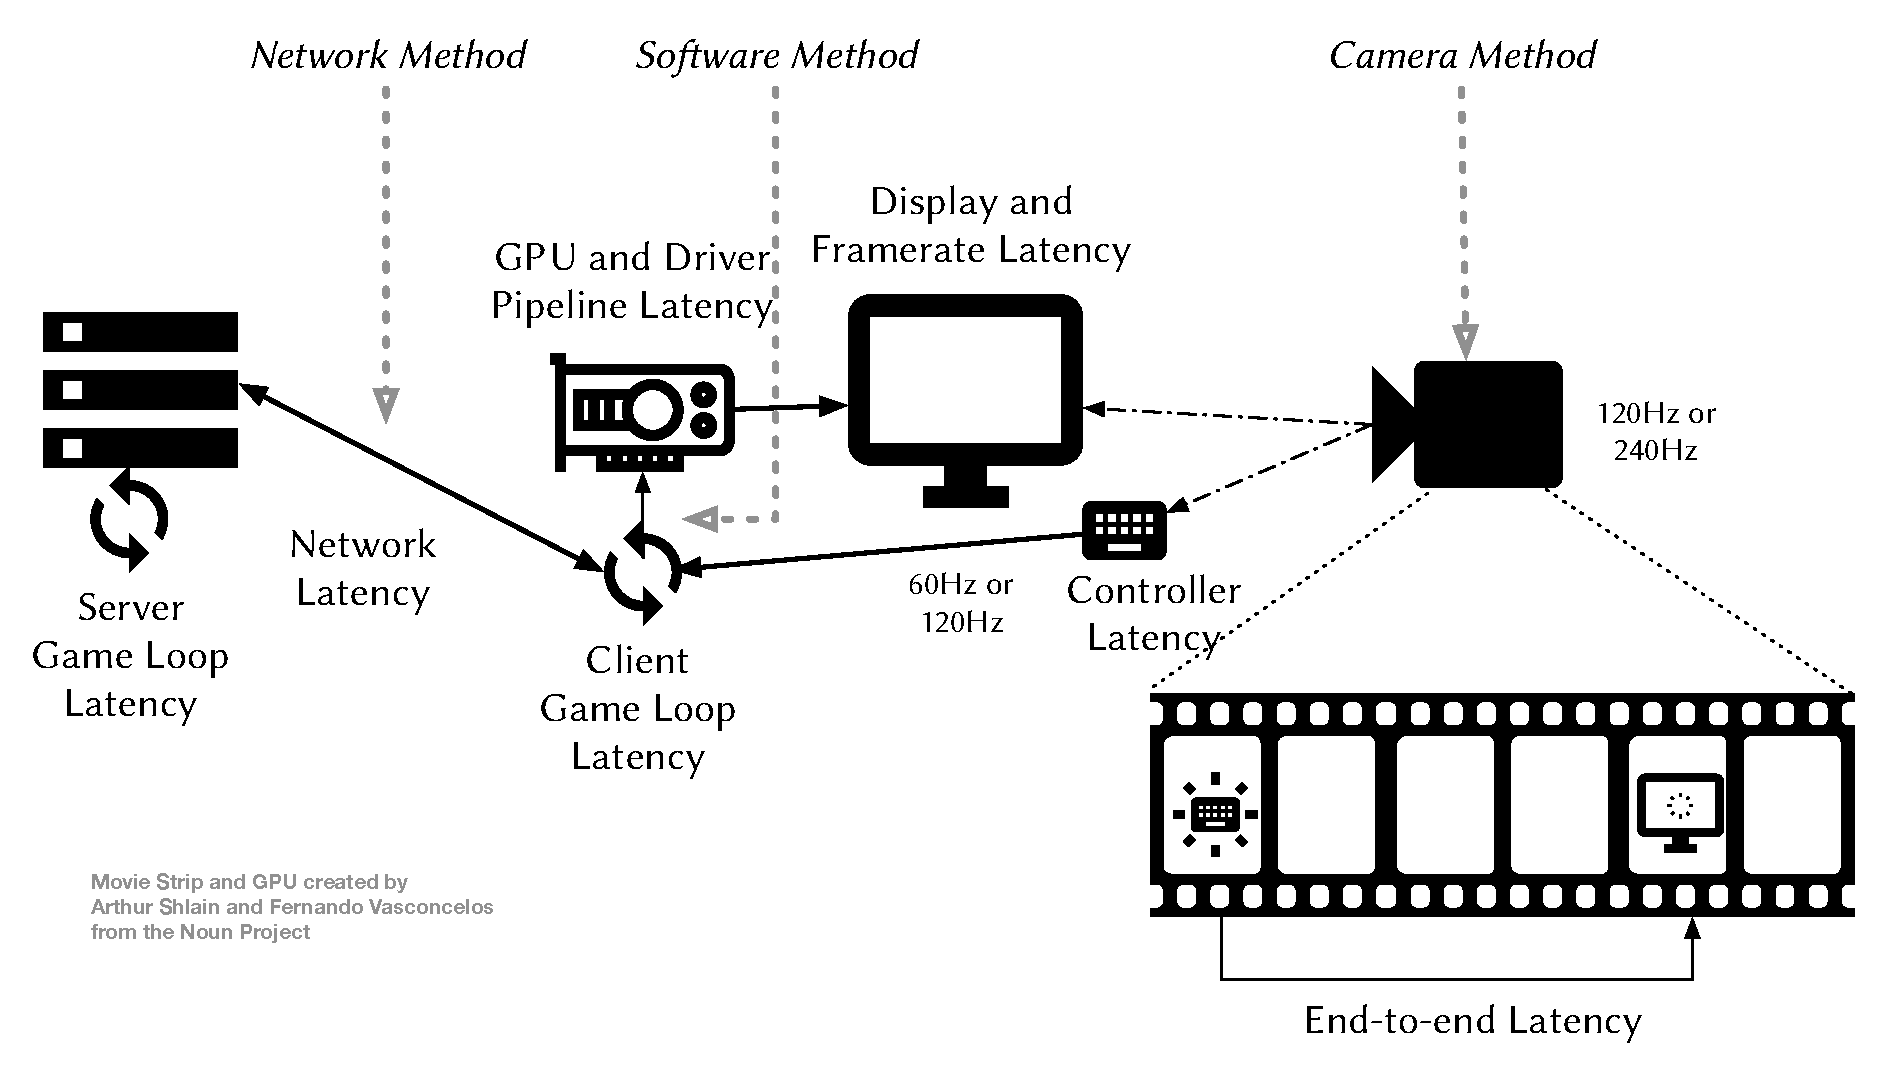
\includegraphics[width=1.0\columnwidth]{../../../models/e2e-lag.pdf}
    \caption{Location of three measurement approaches to capture end-to-end lag in an online video game.}
\label{fig:measurement-methods}
\end{figure}


%%%%%%%%%%%%%%%%%%%%%%%%%%%%%%%%%%%%%%%%%%%%%%%%%%%%%%%%%%%%%%%%%%%%%%%%%%%%%%%%
%\subsection{Related Work}

The outcome of user studies in gaming depends on a wide selection of factors, e.g., on the precise setup, the game, and the choice of players. This makes comparing their results quite difficult. Generalizing the game \acrshort{QoS} and \gls{QoE} assessments and their results has been a topic in past researches, for example correlating online cloud gaming quality with network \acrshort{QoS} (e.g. \cite{5976180}). In order to avoid some of the issues with subjective user studies, other approaches examine the player objective performance through in-game metrics such as the game's highscore or the duration to achieve a certain task. The ``kills per minute'' of players in the \gls{FPS} \textsc{Quake 3} are, for example, investigated by \cite{1266180}, which sees a steady decline of this subjective performance metric when increasing the network delay.
%Finally, an ITU-T Recommendation \cite{mollertowards} concerning subjectively measuring video game \gls{QoE} is also in preparation, which discusses game-relevant \gls{QoS}-metrics as well as the selection of players and games.



\begin{figure}[!t]
	\centering
	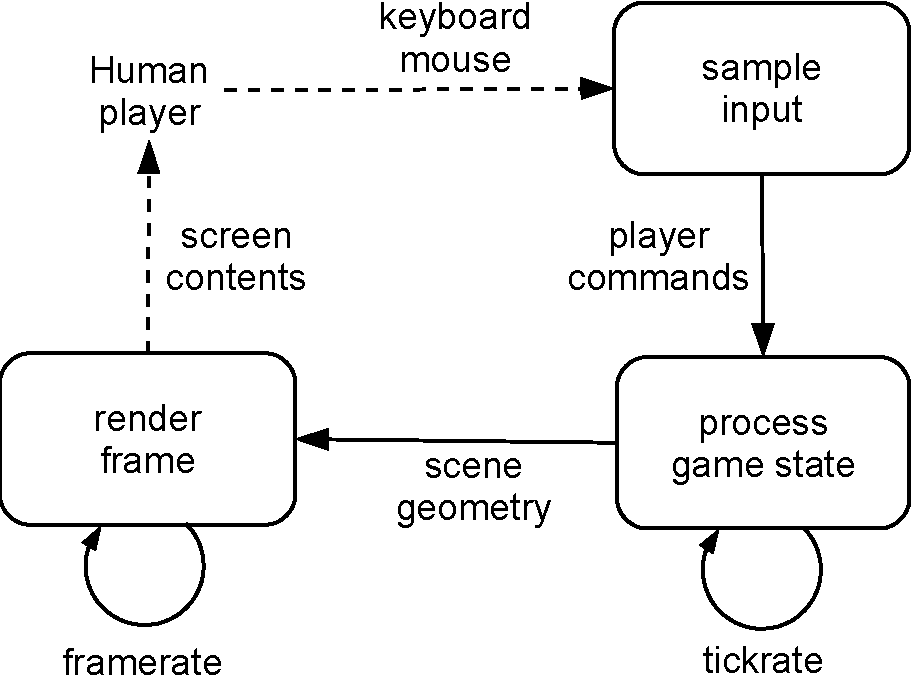
\includegraphics[width=0.8\columnwidth]{../../../models/game_loop.pdf}
	\caption{Basic model of a continuous main video game loop.}
	\label{fig:gameloop1}
\end{figure}

\begin{table}[!t]
\caption{Tickrates in competitive and popular video games that are either known, speculated upon, or derived by counting update and command messages. Data was collected from various sources and should be taken as-is.}
% \hoss{Welche rel. bzw. unreliable sources? Gibt es auch typische framerates dazu?}
% fm: inoffizielle, nicht-wissenschaftliche quellen, da diese werte normalerweise nicht durch den entwickler veröffentlicht werden; für framerates gibt es keine werte, da diese normalerweise unlocked laufen (zumindest für pc, bei konsolen für alle entweder 30 oder 60), ist eigentlich zu komplex um an der stelle darauf einzugehen
\label{tbl:tickrates}
	\centering
	\begin{tabu}{X[0.45]X}
		\toprule
		\textbf{Video Game} & \textbf{Tickrate} \\
		\midrule
		CS: GO & Configurable \SI{64}{\hertz}/\SI{128}{\hertz} \\
		Battlefield 4 & \SI{30}{\hertz}; \SI{10}{\hertz} for state outside of close proximity to player; \SI{60}{\hertz}/\SI{120}{\hertz} on test servers. \\
		Minecraft & max. \SI{20}{\hertz} \\
		League of Legends & \SI{30}{\hertz} (estimated) \\
		Dota 2 & \SI{30}{\hertz} \\
		StarCraft II & supposedly either \SI{16}{\hertz} or \SI{32}{\hertz} \\
		Eve Online & \SI{1}{\hertz} \\
		Project Cars & \SI{600}{\hertz} (Physics), \SI{250}{\hertz} (Input) \\ %https://twitter.com/projectcarsgame/status/551340759858040833
		\bottomrule
	\end{tabu}
\end{table}

\begin{figure*}[!t]
  \centering
  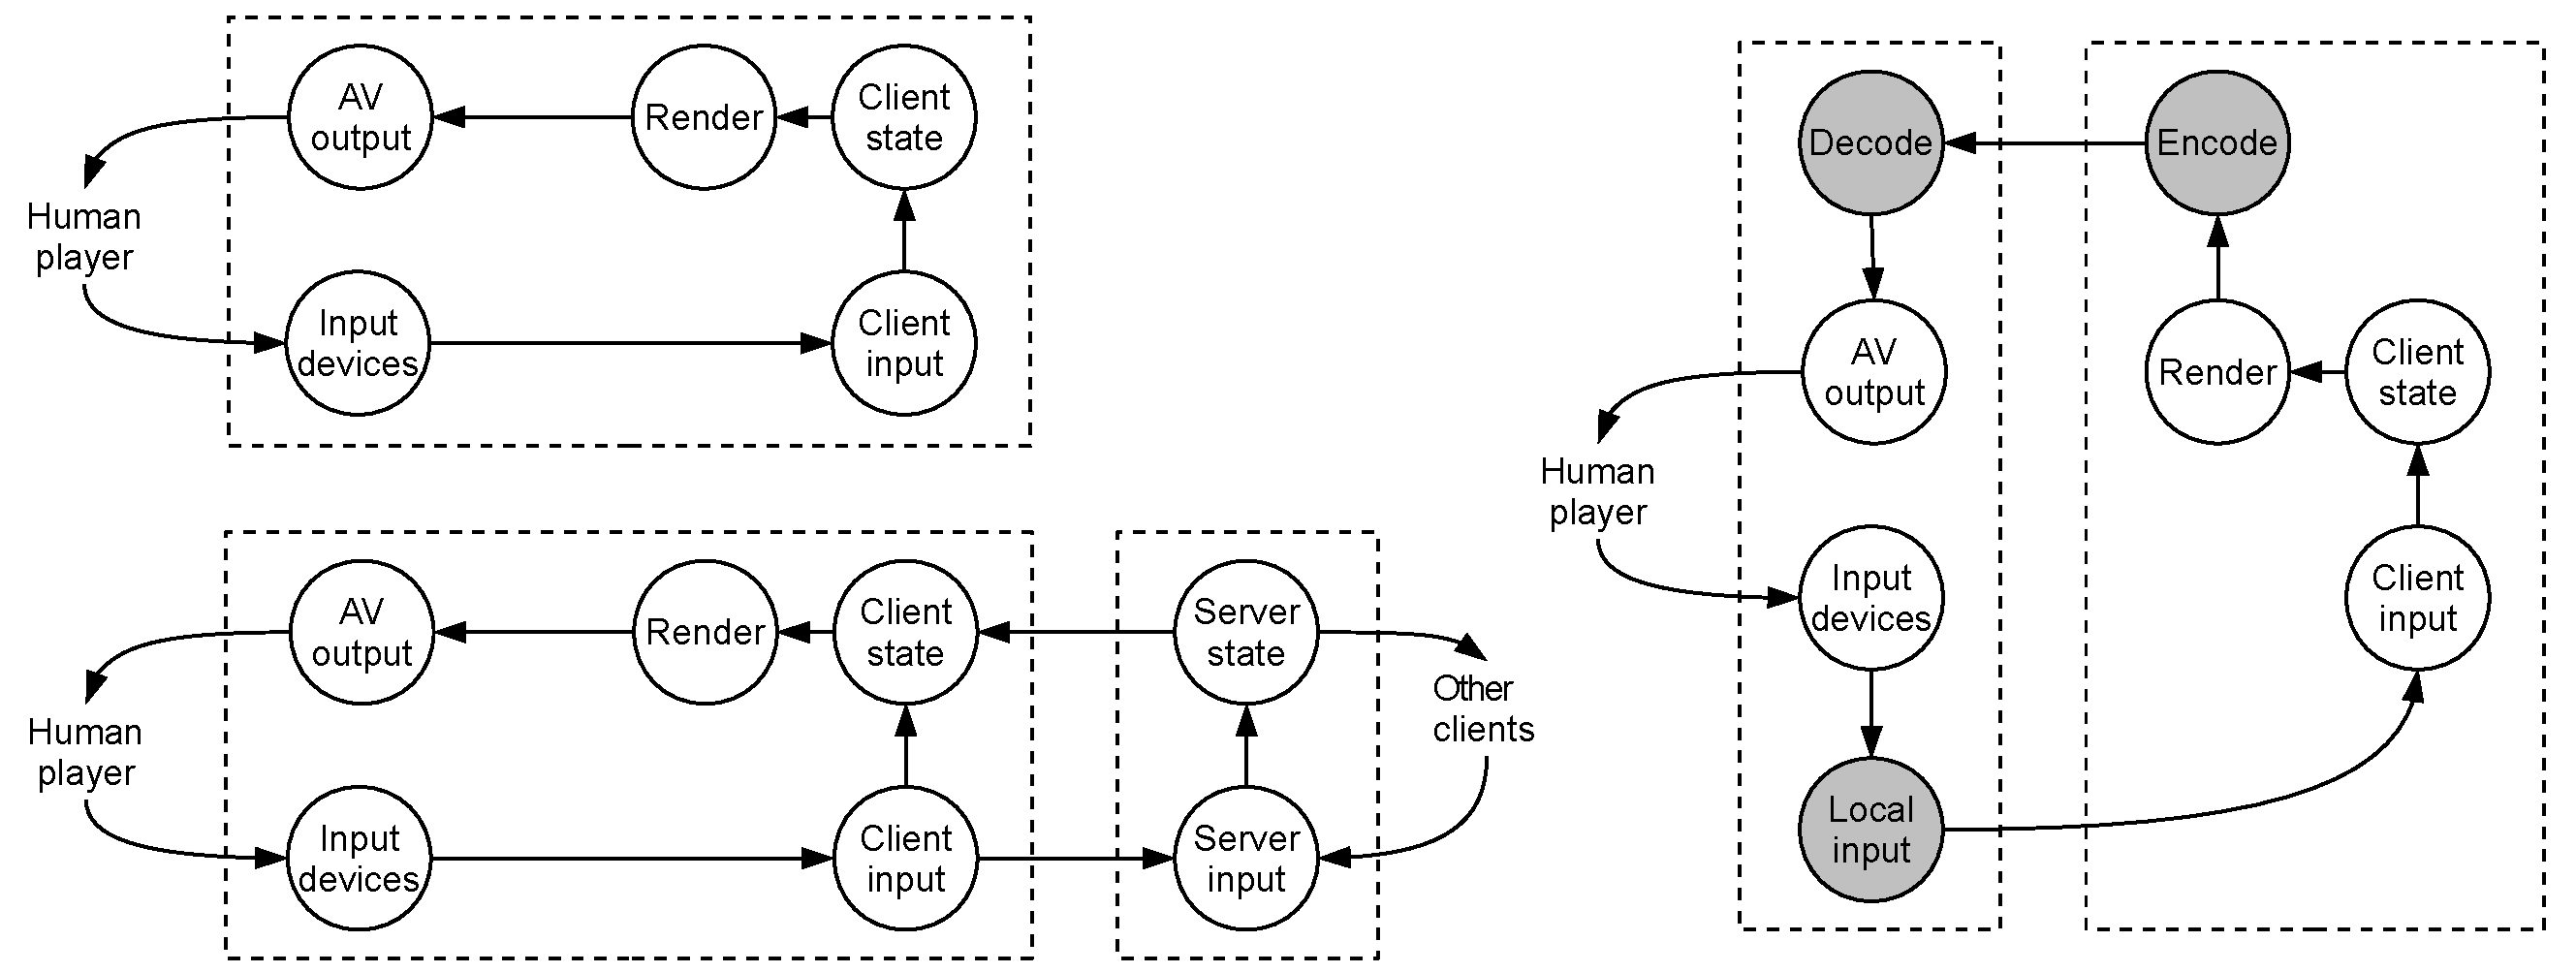
\includegraphics[width=0.9\textwidth]{../../../models/component_interaction_full.pdf}
  \caption{Interactions between components in different video game models. \textit{(a)} Single-player, \textit{(b)} online, \textit{(c)} cloud game.}
  \label{fig:component-models}
\end{figure*}
